% !TEX TS-program = XeLaTeX
% use the following command:
% all document files must be coded in UTF-8
\documentclass[portuguese]{textolivre}
% build HTML with: make4ht -e build.lua -c textolivre.cfg -x -u article "fn-in,svg,pic-align"
\usepackage{array}

\journalname{Texto Livre}
\thevolume{18}
%\thenumber{1} % old template
\theyear{2025}
\receiveddate{\DTMdisplaydate{2025}{7}{3}{-1}} % YYYY MM DD
\accepteddate{\DTMdisplaydate{2025}{8}{26}{-1}}
\publisheddate{\DTMdisplaydate{2025}{9}{28}{-1}}
\corrauthor{Patrick Fernandes Rezende Ribeiro}
\articledoi{10.1590/1983-3652.2025.60103}
%\articleid{NNNN} % if the article ID is not the last 5 numbers of its DOI, provide it using \articleid{} commmand 
% list of available sesscions in the journal: articles, dossier, reports, essays, reviews, interviews, editorial
\articlesessionname{articles}
\runningauthor{Ribeiro e Tsunoda} 
%\editorname{Leonardo Araújo} % old template
\sectioneditorname{Daniervelin Pereira}
\layouteditorname{Saula Cecília}

\title{Geração de textos dinâmicos e criativos com Grandes Modelos de Linguagem (LLMs): uma revisão sistemática}
\othertitle{Generating dynamic and creative texts with Large Language Models (LLMs): a systematic review}
% if there is a third language title, add here:
%\othertitle{Artikelvorlage zur Einreichung beim Texto Livre Journal}

\author[1]{Patrick Fernandes Rezende Ribeiro~\orcid{0000-0002-5973-1110}\thanks{Email: \href{mailto:patrick.ribeiro@ufpr.br}{patrick.ribeiro@ufpr.br}}}
\author[1]{Denise Fukumi Tsunoda~\orcid{0000-0002-5663-4534}\thanks{Email: \href{mailto:dtsunoda@ufpr.br}{dtsunoda@ufpr.br}}}
\affil[1]{Universidade Federal do Paraná, Programa de Pós-Graduação em Gestão da Informação, Departamento de Ciência e Gestão da Informação, Curitiba, PR, Brasil.}


\addbibresource{article.bib}
% use biber instead of bibtex
% $ biber article

% used to create dummy text for the template file
\definecolor{dark-gray}{gray}{0.35} % color used to display dummy texts
\usepackage{lipsum}
\SetLipsumParListSurrounders{\colorlet{oldcolor}{.}\color{dark-gray}}{\color{oldcolor}}

% used here only to provide the XeLaTeX and BibTeX logos
\usepackage{hologo}

% if you use multirows in a table, include the multirow package
\usepackage{multirow}

% provides sidewaysfigure environment
\usepackage{rotating}

% CUSTOM EPIGRAPH - BEGIN 
%%% https://tex.stackexchange.com/questions/193178/specific-epigraph-style
\usepackage{epigraph}
\renewcommand\textflush{flushright}
\makeatletter
\newlength\epitextskip
\pretocmd{\@epitext}{\em}{}{}
\apptocmd{\@epitext}{\em}{}{}
\patchcmd{\epigraph}{\@epitext{#1}\\}{\@epitext{#1}\\[\epitextskip]}{}{}
\makeatother
\setlength\epigraphrule{0pt}
\setlength\epitextskip{0.5ex}
\setlength\epigraphwidth{.7\textwidth}
% CUSTOM EPIGRAPH - END

% to use IPA symbols in unicode add
%\usepackage{fontspec}
%\newfontfamily\ipafont{CMU Serif}
%\newcommand{\ipa}[1]{{\ipafont #1}}
% and in the text you may use the \ipa{...} command passing the symbols in unicode

% LANGUAGE - BEGIN
% ARABIC
% for languages that use special fonts, you must provide the typeface that will be used
% \setotherlanguage{arabic}
% \newfontfamily\arabicfont[Script=Arabic]{Amiri}
% \newfontfamily\arabicfontsf[Script=Arabic]{Amiri}
% \newfontfamily\arabicfonttt[Script=Arabic]{Amiri}
%
% in the article, to add arabic text use: \textlang{arabic}{ ... }
%
% RUSSIAN
% for russian text we also need to define fonts with support for Cyrillic script
% \usepackage{fontspec}
% \setotherlanguage{russian}
% \newfontfamily\cyrillicfont{Times New Roman}
% \newfontfamily\cyrillicfontsf{Times New Roman}[Script=Cyrillic]
% \newfontfamily\cyrillicfonttt{Times New Roman}[Script=Cyrillic]
%
% in the text use \begin{russian} ... \end{russian}
% LANGUAGE - END

% EMOJIS - BEGIN
% to use emoticons in your manuscript
% https://stackoverflow.com/questions/190145/how-to-insert-emoticons-in-latex/57076064
% using font Symbola, which has full support
% the font may be downloaded at:
% https://dn-works.com/ufas/
% add to preamble:
% \newfontfamily\Symbola{Symbola}
% in the text use:
% {\Symbola }
% EMOJIS - END

% LABEL REFERENCE TO DESCRIPTIVE LIST - BEGIN
% reference itens in a descriptive list using their labels instead of numbers
% insert the code below in the preambule:
%\makeatletter
%\let\orgdescriptionlabel\descriptionlabel
%\renewcommand*{\descriptionlabel}[1]{%
%  \let\orglabel\label
%  \let\label\@gobble
%  \phantomsection
%  \edef\@currentlabel{#1\unskip}%
%  \let\label\orglabel
%  \orgdescriptionlabel{#1}%
%}
%\makeatother
%
% in your document, use as illustraded here:
%\begin{description}
%  \item[first\label{itm1}] this is only an example;
%  % ...  add more items
%\end{description}
% LABEL REFERENCE TO DESCRIPTIVE LIST - END


% add line numbers for submission
%\usepackage{lineno}
%\linenumbers

\begin{document}
\maketitle

\begin{polyabstract}
\begin{abstract}
Este artigo apresenta uma revisão sistemática da literatura sobre a aplicação de Grandes Modelos de Linguagem (LLMs) na geração e identificação de textos criativos e dinâmicos com base em referenciais simbólicos, narrativos e do imaginário literário, considerando publicações entre 2014 e 2024. A análise contempla duas etapas principais: (1) triagem e curadoria bibliográfica automatizada com apoio de ferramentas baseadas em inteligência artificial e (2) análise crítica das abordagens, desafios e oportunidades presentes na literatura selecionada. As ferramentas utilizadas permitiram gerenciar referências, extrair metadados e identificar padrões temáticos. Os resultados indicam predominância de estudos voltados à geração criativa de textos e à detecção de linguagem figurada, como metáforas, com uso crescente de modelos híbridos que combinam estruturas simbólicas e subsimbólicas. Conclui-se que, apesar do potencial dos LLMs para a criatividade computacional, persistem desafios como baixa interpretabilidade e escassa adaptação a contextos culturais não hegemônicos.

\keywords{Grandes Modelos de Linguagem\sep Imaginário literário\sep Revisão sistemática}
\end{abstract}

\begin{english}
\begin{abstract}
This article presents a systematic review of the literature on the application of Large Language Models (LLMs) in generating and identifying creative and dynamic texts based on symbolic, narrative, and literary imaginary references, considering publications from 2014 to 2024. The analysis encompasses two main stages: (1) automated bibliographic screening and curation with the support of tools based on artificial intelligence, and (2) critical analysis of the approaches, challenges and opportunities present in the selected literature. The tools used made it possible to manage references, extract metadata, and identify thematic patterns. The results indicate a predominance of studies focused on the creative generation of texts and the detection of figurative language, such as metaphors, with increasing use of hybrid models that combine symbolic and sub-symbolic structures. The conclusion is that, despite the potential of LLMs for computational creativity, challenges persist such as low interpretability and poor adaptation to non-hegemonic cultural contexts.


\keywords{Large Language Models\sep Literary imaginary\sep Systematic review}
\end{abstract}
\end{english}
% if there is another abstract, insert it here using the same scheme
\end{polyabstract}

\section{Introdução}
No campo da Inteligência Artificial (IA), o desenvolvimento de Grandes Modelos de Linguagem \textit{(Large Language Models, LLMs)} mais eficientes, que compreendam, criem e interajam cada vez mais semelhantes à linguagem humana \cite[p. 406]{jurafsky2023} é um campo em contínuo desenvolvimento. Esses modelos conseguem gerar textos, resumir conteúdo, fazer traduções, classificações, categorizações, análises e muito mais; todas essas funcionalidades oferecem ao ser humano um suporte tecnológico para aumentar e melhorar a produtividade, resolver problemas e tomar decisões.

Os LLMs são modelos de linguagem avançados treinados com grande volume de dados. Esses modelos constituem uma especialização dentro do campo da IA com foco no Processamento de Linguagem Natural (PLN) e são fundamentais para IA Generativa (IAG). Utilizando técnicas de aprendizado profundo, eles buscam capturar, dentro do possível, as diferenças sutis e complexidades inerentes à linguagem humana \cite[p. 23]{chang2023}. A partir dessa base conceitual, eles têm demonstrado eficácia em uma variedade de tarefas de PLN, incluindo a geração de texto, tradução automática, reconhecimento de voz, análise de sentimentos e resposta automática a perguntas. No cenário atual, encontra-se, por exemplo, a série GPT \textit{(Generative Pre-trained Transformer)} da OpenAI, o PaLM 2/Bard da Google, o Claude da Anthropic, o Llama 4 da Meta e o DeepSeek.

Apesar desse potencial demonstrado, ainda há limitações e desafios significativos a serem superados pelos LLMs \cite{jovanovic2022}. Entre eles, a questão da qualidade e da coerência dos textos gerados por algoritmos de IAG, que, embora gramaticalmente corretos, muitas vezes, carecem de coesão e profundidade característicos da criatividade humana \cite{santo2023}. Somam-se a isso as ``alucinações" -- respostas geradas que podem ser sem sentido, gramaticalmente incorretas ou factualmente erradas \cite{alkaissi2023} -- como uma preocupação. Ainda que haja curadoria dos dados de treinamento, eles ainda podem produzir saídas inesperadas ou imprecisas, especialmente quando confrontados com \textit{prompts} ambíguos ou fora de seu domínio de treinamento \cite[p. 45]{kaufman2022}.

Como visto, embora LLMs representem avanços na compreensão e geração de linguagem natural, eles ainda enfrentam desafios relacionados à complexidade do uso linguístico humano, pois a comunicação humana é profundamente influenciada por fatores contextuais, sociais e emocionais, como o ambiente, o interlocutor, questões sociais e sentimentos \cite{labov2008, bagno2011, bakhtin2003}. Por exemplo, num contexto de interação comunicativa, seja oral ou escrito, a intenção comunicativa das pessoas muda conforme o interlocutor e o ambiente, e isto tem impacto direto em suas escolhas linguísticas, como na seleção do léxico, estilo, entonação, linguagem ou discurso \cite{bagno2011}. Essas escolhas são normalmente motivadas pelo contexto de uso, como o ambiente profissional, escolar, festivo ou um velório \cite{bakhtin2003, marcuschi2007, bronckart1999, dolz2004}.

O interlocutor, receptor ou destinatário, também exerce influência na forma como a linguagem é usada. O sucesso da comunicação depende da interação entre locutor, receptor, mensagem, canal, código e referente, em uma relação de compreensão e participação ativa do interlocutor. Em situações reais, locutor e receptor trocam frequentemente de papéis e perfis conforme o contexto e o gênero textual \cite{jakobson1976, bakhtin1997, saussure1999, marcuschi2007}.

Além disso, aspectos sociais, como idade, gênero, classe social, nível educacional, também influenciam o modo como as pessoas se expressam \cite{labov2008}. Do mesmo modo, sentimentos como orgulho, carência, paixão, ódio afetam as escolhas linguísticas \cite{bakhtin2003}.

A soma desses fatores -- ambiente, interlocutor, questões sociais e sentimentos -- juntamente com o domínio linguístico, é determinante para a intenção comunicativa, isto é, eles influenciam na forma como as pessoas se expressam e nas escolhas linguísticas que fazem, tornando a linguagem mais ou menos criativa, formal, vulgar, infantil, polida \cite{bagno2011, bakhtin2003}.

Neste contexto, seja na oralidade ou na escrita, a língua adquire dimensões fenomenológicas, pois deixa de ser somente uma estrutura de regras objetivas e passa a ser um fenômeno abstrato, constituído pela experiência vivida -- uma manifestação concreta e intersubjetiva da linguagem \cite{husserl1975, heidegger2012, merleau-ponty1999}. Essa vivência dinâmica e compartilhada da linguagem, como fenômeno vivo, reinventa-se continuamente através da interação social, nos quais a multiplicidade de perfis e papéis sociais permite que intenções discursivas gerem inovações linguísticas, como metáforas; subvertam normas linguísticas por meio do humor e da crítica, como ironias e sarcasmos; e criem variações com neologismos. Por fim, esse processo também gera fenômenos como apropriação linguística (uso de estrangeirismos) e o cruzamento lexical, influenciados por fatores como tecnologia e cultura. Isto resulta na ressignificação da linguagem em novos ambientes, como as redes sociais (ex.: TikTok, WhatsApp), em que surgem neologismos e gírias.

A linguagem natural é dinâmica, criativa e permeada por fenômenos e elementos que desafiam os modelos computacionais a irem além da simples reprodução de padrões probabilísticos, exigindo uma compreensão mais profunda das intenções e das relações sociais subjacentes à comunicação. Portanto, o desenvolvimento de LLMs mais eficientes não é tão-só um desafio técnico, mas também uma busca por aproximar a inteligência artificial da riqueza e complexidade do uso real da linguagem natural.

Pensando nisso, este estudo objetiva realizar uma revisão sistemática estruturada da literatura sobre a aplicação ou a implementação de Grandes Modelos de Linguagem (LLMs) para a identificação ou geração de textos dinâmicos e criativos entre os anos de 2014 e 2024 para responder a seguinte pergunta de pesquisa: ``Quais são as abordagens existentes, os desafios enfrentados e as oportunidades identificadas no uso de Grandes Modelos de Linguagem (LLMs) com referenciais simbólicos, narrativos ou do imaginário literário?".

\section{Grandes modelos de linguagem}
A evolução dos Grandes Modelos de Linguagem (LLMs) representa a popularização da Inteligência Artificial por meio de chats, por exemplo, como GPT. Esses modelos, que hoje ocupam papel central em soluções de automação linguística, têm suas raízes fincadas em décadas de desenvolvimento teórico e técnico que começam nas primeiras tentativas de simular o funcionamento cognitivo humano por meio de redes neurais artificiais. 

O marco fundacional dessa trajetória remonta à década de 1940, quando \textcite{mcculloch1990} propuseram em 1948 um modelo lógico para o funcionamento dos neurônios, estabelecendo as bases para o desenvolvimento de redes neurais. Na década seguinte, o \textit{Perceptron}, de \textcite{rosenblatt1958}, deu início ao uso prático dessas redes em tarefas simples de classificação, inaugurando uma abordagem computacional que buscava replicar, ainda que rudimentarmente, processos de aprendizagem humana.

Contudo, a limitação do \textit{Perceptron} em resolver problemas não-lineares, evidenciada por \textcite{minsky2017perceptrons} em 1969, conduziu ao chamado ``Inverno da IA", um período de descrença e estagnação. Ainda assim, essas dificuldades não impediram a consolidação de uma fundamentação teórica que seria a base para os avanços subsequentes.

O ressurgimento do interesse por redes neurais nas décadas de 1980 e 1990 coincidiu com o desenvolvimento de algoritmos mais eficientes, como a retropropagação \cite{rumelhart1986}, que viabilizou o treinamento de redes multicamadas. Nesse contexto, técnicas mais sofisticadas, como as redes convolucionais (CNNs) e recorrentes (RNNs), demonstraram grande potencial em tarefas como reconhecimento de imagens e processamento de sequências temporais -- componentes críticos para o posterior avanço no Processamento de Linguagem Natural (PLN). A emergência de arquiteturas profundas e o crescimento da capacidade computacional \cite{zhao2003} permitiram não só o aumento do número de parâmetros treináveis, mas também a aplicação de redes neurais em ambientes complexos, como a análise textual em larga escala.

A introdução do \textit{Transformer} por \textcite{vaswani2017} representou um ponto de inflexão na história da IA, ao superar os limites das RNNs e CNNs com um mecanismo de atenção que possibilitou o processamento paralelo e a retenção de contextos distantes em sequências textuais. Essa inovação técnica impulsionou a criação de modelos cada vez maiores, como o BERT \cite{devlin2019}, o GPT-2 \cite{radford2019}, o GPT-3 \cite{brown2020} e, mais recentemente, o GPT-4 \cite{openai2023}. Estes modelos incorporam bilhões de parâmetros e podem executar múltiplas tarefas linguísticas com precisão e fluidez, evidenciando um novo patamar de inteligência algorítmica.

Do ponto de vista dos Estudos da Linguagem, os LLMs não se configuram somente como artefatos tecnológicos avançados, mas, em certa medida, como agentes discursivos que reconfiguram as formas de produção, circulação e apropriação do sentido na sociedade contemporânea. Sua atuação sobre grandes volumes de dados textuais e sua capacidade de gerar respostas contextualizadas ao posicionam como instrumentos potencialmente transformadores nos processos de mediação linguística. No entanto, como apontam \textcite{bender2020}, \textcite{blodgett2020}, \textcite{marcus2020} e \textcite{ortega-martin2023}, os LLMs enfrentam desafios estruturais na compreensão de ambiguidades lexicais e sintáticas, apresentam baixa sensibilidade às variações sociolinguísticas e tendem a reproduzir vieses ideológicos presentes nos dados de treinamento.

Mais especificamente, conforme demonstrado por \textcite{louwerse2011}, sua limitação em interpretar linguagem figurativa e pragmática evidencia a ausência de uma cognição situacional, elemento central nos processos humanos de produção e compreensão de sentido. Tais limitações se somam aos já reconhecidos desafios estruturais, como o alto custo computacional, os riscos de viés algorítmico \cite{bender2021} e os dilemas éticos relacionados à privacidade, transparência e responsabilidade social. Assim, uma compreensão crítica e inter/transdisciplinar dos LLMs é imprescindível.

\section{Metodologia}
O presente estudo segue uma metodologia de revisão sistemática da literatura para apresentar e identificar as abordagens existentes, os desafios e as oportunidades na intersecção entre LLMs e o imaginário literário. A análise abarca publicações acadêmicas entre 2014 e 2024.

Para tanto, o encaminhamento metodológico é composto por etapas que compreendem desde a formulação de uma pergunta estruturada de pesquisa até a análise detalhada dos documentos recuperados, passando por seleção de fontes de dados e triagem dos artigos.

Especificamente, o objetivo é identificar as tendências emergentes que exploram a implementação ou análise do uso de referenciais simbólicos, narrativos e do imaginário literário em LLMs.

\subsection{Materiais}
A etapa de análise dos artigos e a extração das informações bibliométricas contemplou a utilização das seguintes ferramentas que usam inteligência artificial:

\begin{itemize}
    \item Zotero (v.7.0.15): organização de referências, remoção de duplicatas e exportação em BibTeX;
    \item OpenAlex: extração de metadados (palavras-chave, citações, ano, periódico);
    \item Rayyan: remoção complementar de duplicatas e triagem dos artigos;
    \item Biblioshiny: análise bibliométrica exploratória;
    \item NotebookLM: leitura e análise de PDFs;
    \item SciSpace (versão paga): análise automatizada do texto completo;
    \item Litmaps: visualização de redes de citações;
    \item ChatGPT (versão paga): apoio à análise de conteúdo e identificação de tendências;
\end{itemize}

A opção pela utilização destas ferramentas neste estudo se justifica na contribuição ao processo de organização e construção do conhecimento, também por critérios técnicos de desempenho. Assim, cabe reforçar o papel complementar que desempenhou cada ferramenta no processo de revisão sistemática.

Ferramentas como Zotero e Rayyan mostraram-se fundamentais na curadoria bibliográfica, garantindo confiabilidade na gestão das fontes e consistência na triagem dos artigos. O ChatGPT foi utilizado como assistente para a identificação de padrões conceituais e na estruturação temática dos resultados. Já NotebookLM e SciSpace deram suporte à extração contextualizada de informações como, por exemplo, LLMs e datasets utilizados, por permitirem a leitura e análise dos textos completos.

Portanto, cada uma dessas ferramentas contribuiu para o rigor metodológico da pesquisa, assegurando a coerência interpretativa dos resultados. As próximas seções detalham o uso dessas ferramentas nas diversas etapas da pesquisa.

\subsection{Estratégia de pesquisa}
Para a estratégia de busca, foi formulada uma pergunta que orientou toda a revisão sistemática. Utilizou-se o \textit{framework} SPICE, desenvolvido para pesquisas em ciências sociais aplicadas.

O SPICE constitui um mnemônico proposto por \textcite{booth2006} como adaptação do \textit{framework} PICO \cite{crumley2002}, voltado especialmente para áreas como biblioteconomia e outras ciências sociais. A aplicação deste \textit{framework} na formulação da pergunta está detalhada na Tabela \ref{tab-1}.

%--- código da tabela 1 ---%
\begin{table}[ht!]
\centering
\begin{threeparttable}
\caption{Definição da pergunta estrutura de pesquisa com \textit{framework} SPICE.}\label{tab-1}
\begin{tabularx}{\textwidth}{l X}
\toprule
Elemento & Conteúdo da Revisão Sistemática \\
\midrule
S - Setting & Produção entre 2014 e 2024, sobre LLMs em contexto de imaginário literário. \\
P - Perspective & Pesquisadores, estudiosos em Inteligência Artificial e literatura. \\
I - Intervention & Uso e análise de LLMs com referenciais simbólicos, narrativos ou do imaginário literário. \\
C - Comparison & Diferentes abordagens metodológicas, epistemológicas ou teóricas nessa intersecção. \\
E - Evaluation & Identificação de abordagens, desafios, oportunidades e tendências emergentes. \\
\bottomrule
\end{tabularx}
\source{Elaborado pelos autores.}
\end{threeparttable}
\end{table}

A partir da pergunta estruturada, desenvolveu-se a estratégia de busca com descritores que abrangem tanto os LLMs quanto os principais conceitos relacionados ao imaginário literário. A escolha dos termos visou garantir a recuperação de estudos relevantes e alinhados à pergunta de pesquisa.

A expressão de pesquisa utilizada foi: ``(``large language models" OR llm OR llms OR ``modelos de linguagem grandes" OR ``modelos de linguagem extensos" OR ``modelos de linguagem de grande porte") AND (imagination OR imaginação OR symbolism OR simbolismo OR symbol OR símbolo OR poetics OR poética OR literature OR literatura OR poetry OR poesia OR poem OR poema OR imaginary OR imaginário OR symbolic OR simbólico OR metaphor OR metáfora OR metaphorical OR metafórico))".

Além disso, foram adotados os seguintes parâmetros de filtragem: artigos de acesso aberto publicados entre 2014 e 2024, em inglês, espanhol ou português.

A base OpenAlex foi selecionada como fonte primária desta revisão sistemática por atender aos critérios metodológicos do estudo: acesso aberto, integração de fontes relevantes, exportação em formatos compatíveis com ferramentas como o Biblioshiny e atualização contínua de seus registros. Seu principal diferencial é o uso de inteligência artificial para a desambiguação de autores e instituições, bem como na classificação semântica dos artigos por \textit{embeddings}, ampliando a precisão na organização e análise dos dados. Essas funcionalidades a tornam adequada aos objetivos da pesquisa.

A coleta de dados foi realizada em 30 de abril de 2025, com 2.506 registros recuperados\footnote{Link de acesso ao conjunto de dados coletados: \url{https://zenodo.org/records/15800742}.}.

\subsection{Critérios de inclusão e exclusão}

A definição dos critérios de inclusão e exclusão foi elaborada com base nos objetivos específicos da revisão sistemática, buscando garantir a relevância, a qualidade e a adequação metodológica dos estudos selecionados. A seguir, detalham-se os critérios adotados na Tabela \ref{tab-2}:

%--- código da tabela 2 ---%
\begin{table}[h!]
\centering
\begin{threeparttable}
\caption{Critérios de Inclusão e de Exclusão.}\label{tab-2}
\small
\begin{tabularx}{\textwidth}{X X}
\toprule
Critérios de Inclusão & Critérios de Exclusão \\
\midrule
Estudos que abordem diretamente Grandes Modelos de Linguagem. & Trabalhos focados apenas em modelos estatísticos ou linguísticos tradicionais, sem uso de redes neurais ou \textit{transformers}. \\
\addlinespace
Análise ou uso de referenciais do imaginário literário, narrativo ou simbólico (ex: metáfora, ironia, sarcasmo). & Estudos sem conexão com o imaginário ou a construção de sentido. \\
\addlinespace
Investigação de aspectos como sentido, coerência, fluidez textual, criatividade e construção narrativa em LLMs. & Textos sem revisão por pares, incompletos ou com acesso restrito. \\
\addlinespace
Intervalo: entre 2014 e 2024. & Publicações fora do intervalo definido. \\
\addlinespace
Textos completos, disponíveis em acesso aberto e passíveis de \textit{download}. & Documentos inacessíveis, com \textit{paywall} ou apenas com resumos disponíveis. \\
\addlinespace
Idiomas português, inglês ou espanhol. & Textos em idiomas diferentes dos definidos. \\
\addlinespace
Gênero textual: artigo científico ou \textit{preprint}. & Outros gêneros textuais diferentes dos definidos. \\
\addlinespace
Palavras-chave associadas: \textit{Large Language Model}, \textit{Large Language Models}, LLM, LLMs. & Trabalhos sem menção ou relação com LLMs nos descritores ou no conteúdo. \\
\bottomrule
\end{tabularx}
\source{Elaborado pelos autores.}
\end{threeparttable}
\end{table}

\subsection{Fluxo de seleção e análise}

A triagem inicial dos estudos utilizou a base OpenAlex, que disponibiliza dados em acesso aberto e estruturado, contemplando publicações de 2014 a 2024. Os dados foram exportados em formato CSV e importados para o gerenciador de referências Zotero. Nessa fase, aplicaram-se rotinas automatizadas de detecção e remoção de registros duplicados e inacessíveis, acelerando o descarte de publicações irrelevantes ou redundantes. Após essa filtragem preliminar, restaram 2.497 artigos únicos.

Em seguida, os registros foram importados para o Rayyan, plataforma especializada em triagem sistemática colaborativa. O sistema detectou 409 possíveis duplicações adicionais. Mediante análise criteriosa, constatou-se que somente 205 registros estavam efetivamente duplicados, sendo removidos do corpus. As demais ocorrências, embora similares, não configuravam duplicidade literal. Ao final dessa etapa, obteve-se um conjunto de 2.292 artigos únicos.

Na fase de \textit{screening}, analisaram-se os títulos, resumos e palavras-chave dos 2.292 artigos. A análise seguiu abordagem híbrida: com o apoio do ChatGPT combinado com leitura manual por pesquisador do grupo. Em casos duvidosos, aplicou-se um procedimento de \textit{blind review} conduzido por outro pesquisador, garantindo maior rigor metodológico. Ao término desta etapa, 2.235 publicações foram excluídas, restando 57 consideradas potencialmente elegíveis.

A etapa seguinte consistiu na leitura integral \textit{(full-text screening)} dos 57 documentos selecionados, reaplicando-se os critérios de inclusão e exclusão. A leitura contou com o suporte das ferramentas SciSpace e NotebookLM, que auxiliaram na extração e organização das informações relevantes. Como resultado, 16 publicações foram excluídas, totalizando 41 selecionadas para análise final.

Os 41 documentos foram analisados em profundidade, com foco nos seguintes aspectos: modelos de LLM utilizados, abordagens narrativas e simbólicas adotadas, objetivos dos estudos, metodologias aplicadas e contribuições identificadas. Os arquivos PDF foram inseridos no Zotero para exportação em formato BibTeX, uma vez que o Rayyan não gera arquivos compatíveis com o Biblioshiny, ferramenta utilizada nas análises bibliométricas. Complementarmente, utilizou-se a ferramenta Litmaps para análise visual de redes de referências e citações.

A análise dos dados seguiu abordagem integrada, contemplando dimensões qualitativas e quantitativas. A dimensão qualitativa concentrou-se na leitura interpretativa dos textos, visando compreender as abordagens adotadas, os desafios relatados e as oportunidades teóricas e aplicadas em torno do uso de LLMs em contextos simbólicos, narrativos e do imaginário literário. A dimensão quantitativa envolveu métricas bibliométricas relacionadas à distribuição temporal das publicações, frequência de ocorrência de determinados modelos de LLM e análise de coocorrência de palavras-chave, permitindo identificar tendências emergentes e lacunas de pesquisa na literatura.

\section{Resultados e análise}

A Figura \ref{fig-1} a seguir ilustra a evolução temporal da produção acadêmica sobre o uso de LLMs com referenciais do imaginário literário, simbólico ou narrativo no período de 2014 a 2024. A figura revela uma tendência de crescimento exponencial que se inicia apenas em 2022, com um período de ausência de publicações entre 2014 e 2021. Esta lacuna inicial indica que a intersecção entre LLMs e estudos literários/simbólicos é um campo de pesquisa emergente e relativamente recente.

%--- código da figura 1 ---%
\begin{figure}[htbp]
\centering
\begin{minipage}{0.65\textwidth}
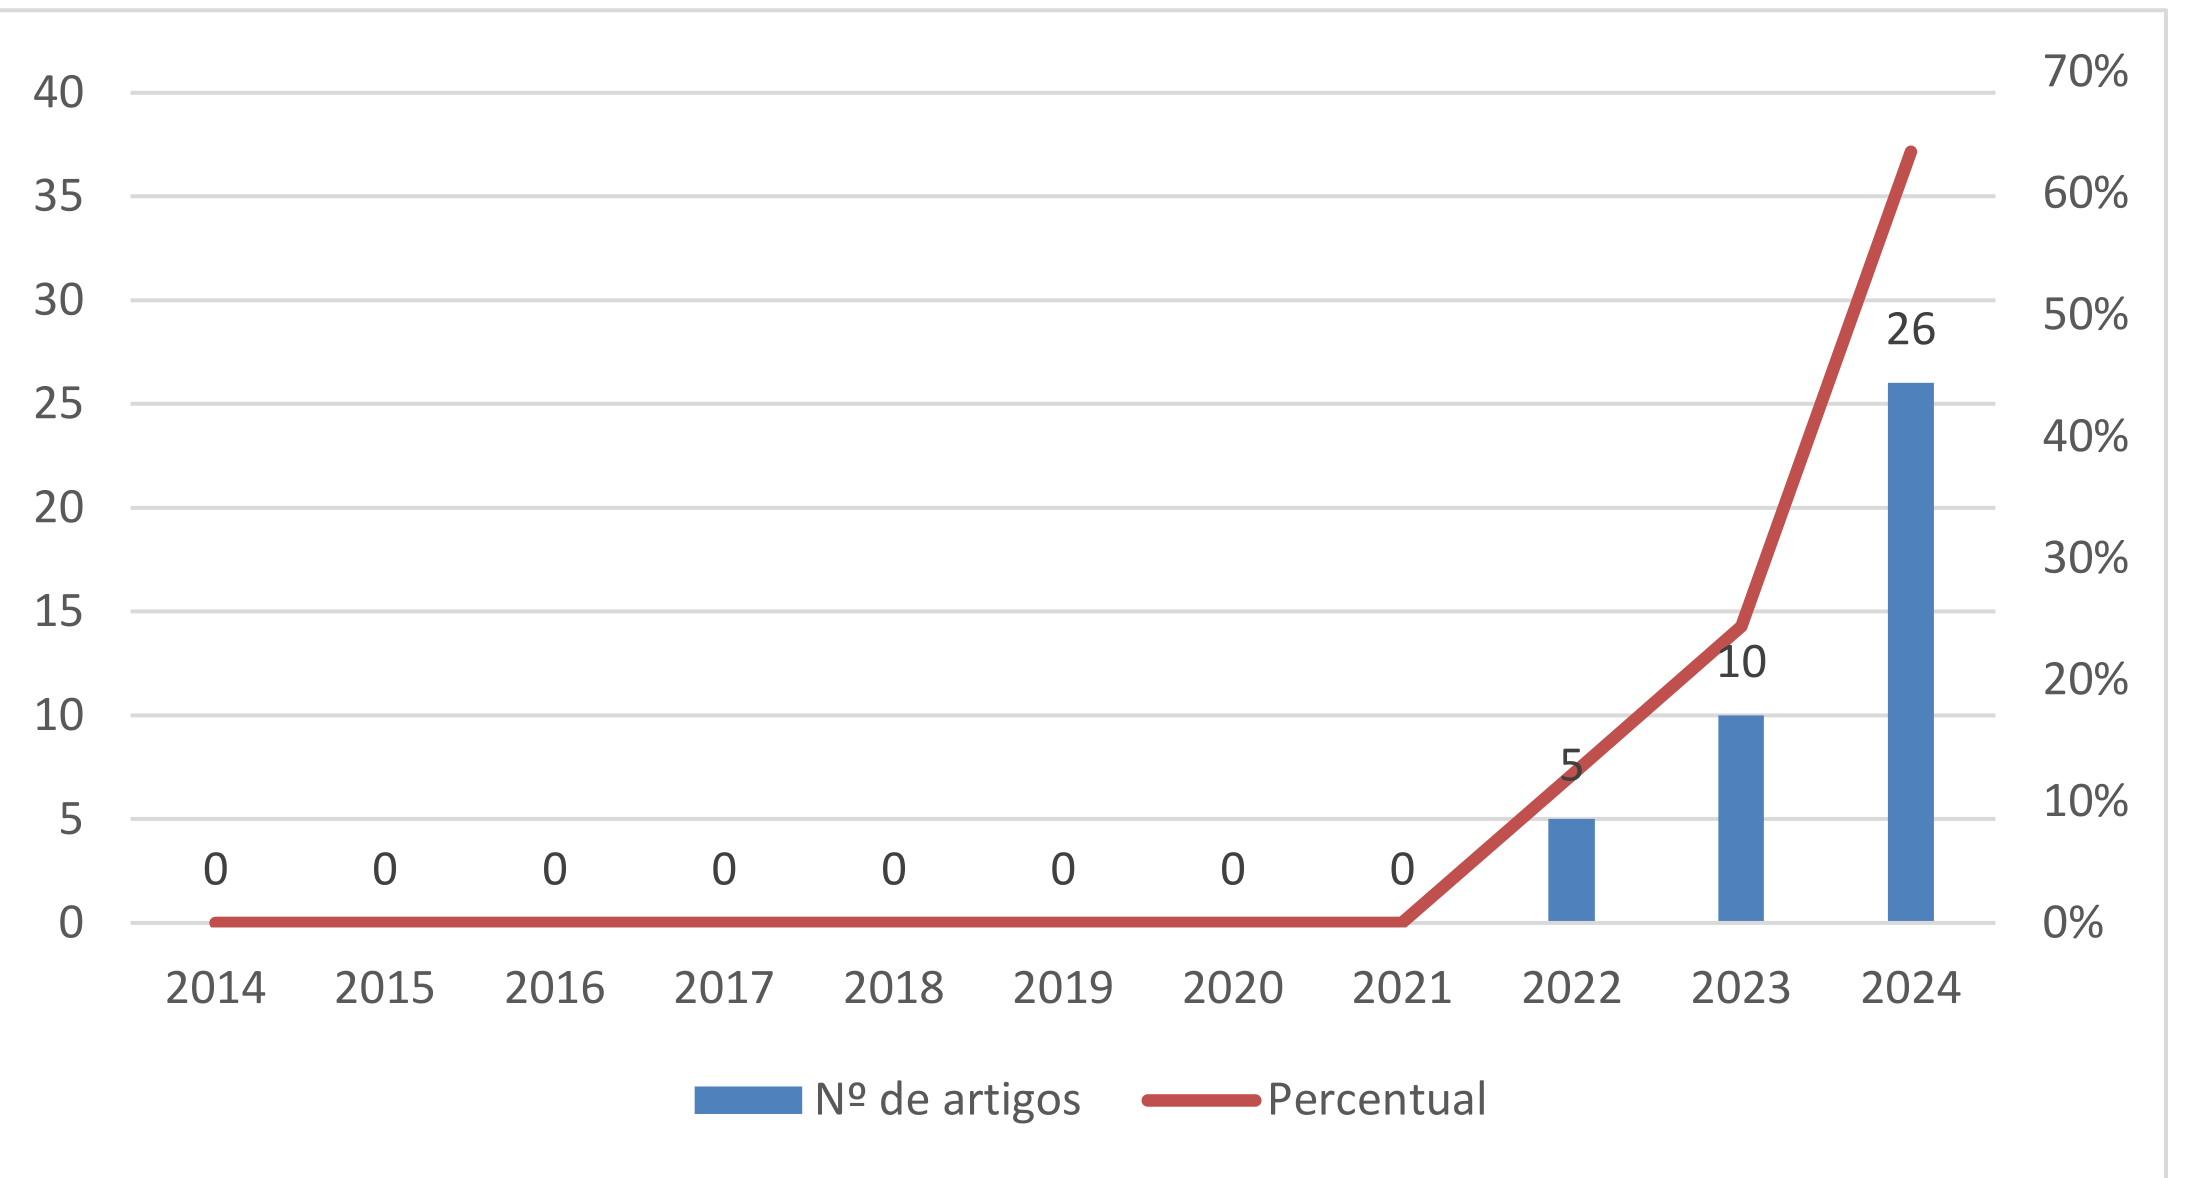
\includegraphics[width=\textwidth]{Imagens/fig-001.png}
\caption{Publicações sobre LLMs com referenciais do imaginário literário, simbólicos ou narrativos no período de 2014 a 2024.}
\label{fig-1}
\source{Elaborado pelos autores.}
\end{minipage}
\end{figure}

O crescimento expressivo da produção acadêmica sobre LLMs com referenciais do imaginário literário, simbólicos ou narrativos entre 2022 e 2024 (Figura \ref{fig-1}) está diretamente relacionado a avanços tecnológicos, à popularização dos modelos e às novas aplicações interdisciplinares.

Em 2022, foram publicados 5 artigos, refletindo o início do interesse acadêmico em explorar as possibilidades dos LLMs para análise simbólica e literária. Esse número ainda representava uma fração pequena da produção total, visto que a tecnologia começava a se consolidar para além das áreas técnicas. Este movimento coincide com o lançamento do ChatGPT pela OpenAI em novembro de 2022, baseado no modelo GPT-3.5. Desde então, o uso de LLMs se tornou amplamente acessível, popularizando aplicações de IA em linguagem natural, inclusive em áreas de humanidades e literatura. Paralelamente, empresas como a Google anunciavam o PaLM, e a DeepMind lançava o Gopher, enquanto a comunidade científica especulava sobre o desempenho do então aguardado GPT-4.

Em 2023, o número de artigos aumentou para 13, indicando que mais pesquisadores passaram a aplicar LLMs em estudos de literatura, simbolismo e imaginário. Isso se deve, em parte, à capacidade desses modelos de analisar grandes volumes de texto e identificar padrões narrativos e simbólicos complexos.

Esse crescimento está atrelado à ampliação das capacidades dos modelos. O lançamento do GPT-4, em março de 2023, trouxe avanços significativos em compreensão contextual, geração de texto e capacidade multimodal. Outros modelos contribuíram também para esse cenário, como LLaMA (Meta), PaLM2 (Google), além de versões \textit{open-source} que ampliaram as possibilidades de experimentação e personalização, por parte da comunidade acadêmica. A partir disso, observou-se uma tendência crescente de estudos que investigam a convergência entre IA simbólica e conexionista, com LLMs sendo utilizados para raciocínio simbólico e integração com estruturas de conhecimento, como grafos e ontologias.

O ano de 2024 registra o pico da série histórica, concentrando 55\% da produção total do período. Este crescimento está associado ao lançamento de modelos como GPT-4o, Gemini 2.0, LLaMA 3.2 e Claude 3.5 Sonnet. Destaca-se também a consolidação dos modelos \textit{open-source}. Esses avanços permitiram maior experimentação e adaptação para tarefas específicas, incluindo análise simbólica e narrativa em literatura. Além disso, a demanda pela comunidade científica por ferramentas de explicabilidade e pelas discussões sobre viés e ética tornou-se central. Isso é especialmente relevante em áreas sensíveis como literatura, história e ciências humanas, incentivando abordagens metodológicas mais robustas.

A análise bibliométrica, conduzida com o auxílio do Biblioshiny, revelou um total de 142 autores distintos, com uma média de 3,46 autores por documento, indicando uma tendência predominante à produção científica colaborativa no campo investigado. Ainda assim, foram identificados seis artigos de autoria individual, demonstrando haver espaço para contribuições independentes.

No que se refere ao impacto da produção, o \textit{corpus} analisado apresenta um total de 3.017 referências distribuídas entre 81 fontes, com uma média de 11,28 citações por artigo. O mapa temático da Figura \ref{fig-2}, gerado a partir da coocorrência de palavras-chave no Biblioshiny, fornece uma visualização estruturada dos principais eixos conceituais que permeiam a literatura, permitindo observar como os temas se inter-relacionam e evoluem ao longo do período analisado.

%--- código da figura 2 ---%
\begin{figure}[htbp]
\centering
\begin{minipage}{0.90\textwidth}
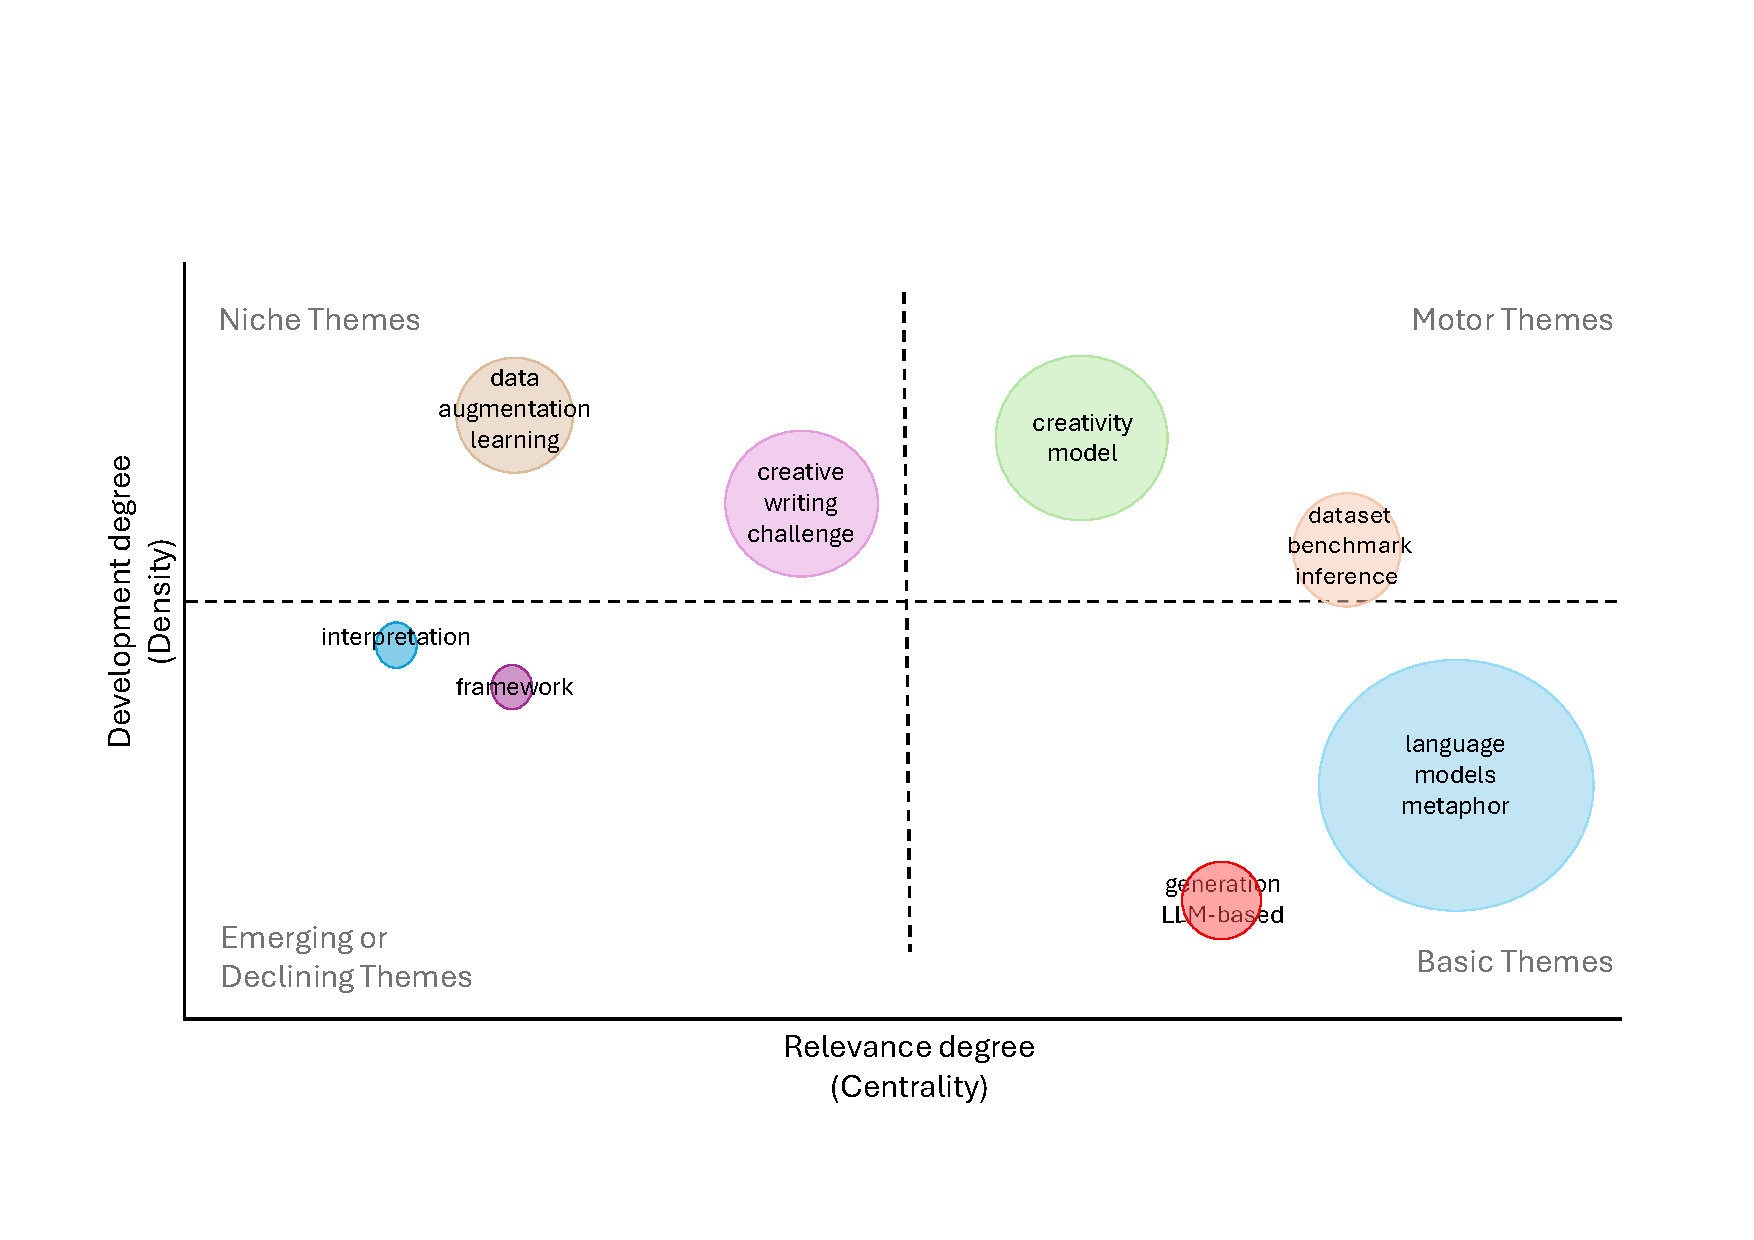
\includegraphics[width=\textwidth]{Imagens/fig-002.pdf}
\caption{Mapeamento temático da literatura por coocorrência de palavras-chave no Biblioshiny.}
\label{fig-2}
\source{Dados da pesquisa.}
\end{minipage}
\end{figure}

O mapa temático (Figura \ref{fig-2}) classifica os principais temas da literatura sobre LLMs com referenciais simbólicos, narrativos ou do imaginário literário (2014-2024), distribuindo-os em quatro quadrantes conforme seu nível de desenvolvimento (densidade) e relevância (centralidade). Nota-se que o tópico \textit{``language models metaphor"} sobressai como um tema fundamental e central para a área, embora ainda se encontre em processo de desenvolvimento. No quadrante dos temas motores -- centrais e bem desenvolvidos -- aparecem \textit{``creativity model"} e \textit{``dataset benchmark inference"}, indicando áreas consolidadas e de grande influência na literatura.

Por sua vez, \textit{“data augmentation learning”} e \textit{“creative writing challenge”} figuram como nichos especializados: bem desenvolvidos, mas pouco conectados ao núcleo central da área. Já \textit{“interpretation”} e \textit{“framework”} aparecem como temas emergentes ou em declínio, com baixa centralidade e desenvolvimento. Finalmente, \textit{“generation LLM-based”} posiciona-se próximo ao eixo central, sugerindo relevância moderada, porém ainda em fase de consolidação.

A Figura \ref{fig-3} apresenta os resultados obtidos via Litmaps, que evidenciam a organização dos artigos científicos segundo seu número de citações. O Litmaps \textit{(Literature Map)} constitui recurso visual interativo que representa a literatura acadêmica por meio de nós (artigos) e conexões que expressam relações conceituais, temáticas ou de citação entre os documentos.

 A análise do mapa revela que, entre os dez artigos mais citados, há predomínio de pesquisadores vinculados a instituições dos Estados Unidos (três artigos) e da China (dois artigos), indicando a centralidade desses países na produção científica de maior impacto sobre o tema investigado.  Destaca-se, ainda, a presença de autores oriundos da Austrália, Espanha, Coreia do Sul, Itália e Índia entre as demais publicações altamente citadas, evidenciando a disseminação e o interesse global pela temática, transcendente a contextos nacionais específicos.

Cabe ressaltar que dentre os 41 artigos analisados, não foi identificado nenhum autor brasileiro ou vinculado a instituições brasileiras.

%--- código da figura 3 ---%
\begin{figure}[htbp]
\centering
\begin{minipage}{0.90\textwidth}
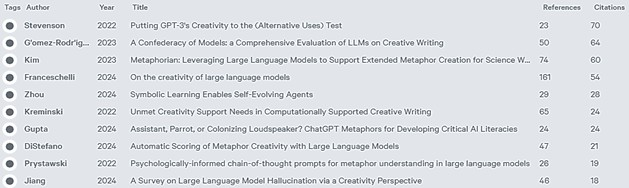
\includegraphics[width=\textwidth]{Imagens/fig-003.jpg}
\caption{Artigos ordenados por ordem de citação no Litmaps.}
\label{fig-3}
\source{Dados da pesquisa.}
\end{minipage}
\end{figure}

A análise bibliométrica realizada com o Litmaps revelou que “Putting GPT-3's Creativity to the (Alternative Uses) Test” \cite{stevenson2022} ocupa uma posição central na rede de cocitações dos 41 documentos selecionados para esta revisão sistemática. Sua relevância se evidencia tanto pelo número de conexões estabelecidas quanto pelo grau de influência em publicações subsequentes (Figura \ref{fig-3}).

Entre os documentos relacionados, destacam-se duas publicações de Giorgio Franceschelli e Mirco Musolesi: ``On the Creativity of Large Language Models" \citeyear{franceschelli2024} e ``Creativity and Machine Learning: A Survey" \citeyear{franceschelli2021}. Ambos os artigos contribuem para a delimitação do campo de estudos sobre criatividade computacional, sendo frequentemente cocitados com o trabalho de \textcite{stevenson2022}.

A primeira publicação analisa se modelos como o GPT-3 podem gerar respostas criativas e inovadoras que resolvam problemas de forma eficaz, indo além da mera reprodução de padrões existentes. A segunda constitui uma revisão abrangente da intersecção entre aprendizado de máquina e criatividade, abordando desde fundamentos teóricos até aplicações práticas e implicações sociais.

O trabalho de \textcite{stevenson2022} concentrou-se em testar a capacidade criativa do GPT-3 em comparação com seres humanos, usando o Teste de Usos Alternativos de Guilford (AUT) -- um método clássico para medir criatividade. Os pesquisadores compararam as respostas geradas pelo GPT-3 com as de humanos (estudantes de psicologia) considerando quatro dimensões: originalidade, utilidade, surpresa e flexibilidade.

Os resultados evidenciam que, embora o GPT-3 produza respostas consideradas mais úteis, às respostas humanas foram atribuídas maior originalidade, surpresa e flexibilidade. O estudo também empregou uma métrica automatizada baseada na distância semântica para avaliar a criatividade. Apesar de o GPT-3 ainda apresentar desempenho inferior aos humanos na maioria dos aspectos, os pesquisadores acreditam que melhorias futuras poderão superar essas limitações.

O trabalho discute o que essas diferenças revelam sobre a criatividade humana em comparação à inteligência artificial, levantando reflexões sobre como definir e mensurar criatividade na atualidade.

A Figura \ref{fig-4}, gerada pelo Litmaps, ilustra visualmente essas conexões, demonstrando como o artigo de \textcite{stevenson2022} articula-se com uma produção científica recente.

%--- código da figura 4 ---%
\begin{figure}[htbp]
\centering
\begin{minipage}{0.90\textwidth}
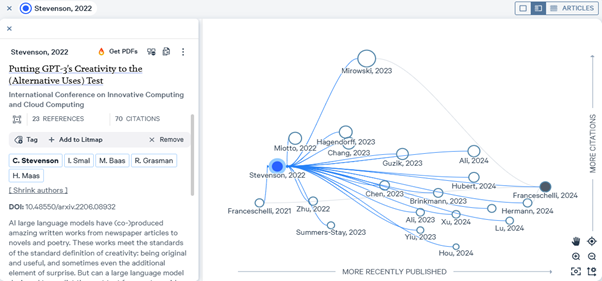
\includegraphics[width=\textwidth]{Imagens/fig-004.png}
\caption{Mapa de cocitações do artigo ``Putting GPT-3's Creativity to the (Alternative Uses) Test'' \cite{stevenson2022}, gerado com Litmaps.}
\label{fig-4}
\source{Dados da pesquisa.}
\end{minipage}
\end{figure}

A análise estruturada realizada via SciSpace possibilitou identificar os LLMs mencionados nos 41 artigos selecionados para esta revisão. A extração automatizada das ocorrências revelou a diversidade de arquiteturas e abordagens empregadas nas pesquisas recentes. Dentre os LLMs identificados estão: 
ALBERT, Alpaca, BART, BERT, Bard, Bing Chat, ChatGPT,
Chinese Tiny LLM, Claude-1.2, Claude-3.5, CodeBERT,
CroSloEngual BERT (CSE BERT), DeBERTa, DeBERTa-V3,
DialoGPT-medium, Dolly 2.0, Gemma-2,
GPT-2, GPT-3, GPT-3.5, GPT-4, GPT-4V, GPT-4o,
GPT-Neo, GPT-NeoX, GPT4All-J, Koala,
LLaMA, LLaMA 2, LLaMA 3, LLaMA 3.1, LLaVA,
MAP-NEO, MOSS, OPT, OpenAssistant, PaLM,
Qwen2, Qwen2\text{-}plus, RoBERTa, SBERT\_MiniLM, SBERT\_mpnet, 
SimCSE, SloBERTa, StableLM, T5, UnifiedQA, Vicuna, XLM-R, Yi-1.5,
mBERTBASE e mT5. Essa variedade reflete o ecossistema dinâmico de desenvolvimento e aplicação dos LLMs nos últimos anos.

A Figura \ref{fig-5} apresenta os 10 modelos mais utilizados nas publicações analisadas, indicando tendências de adoção e preferência no cenário acadêmico contemporâneo.

%--- código da figura 5 ---%
\begin{figure}[htbp]
\centering
\begin{minipage}{0.75\textwidth}
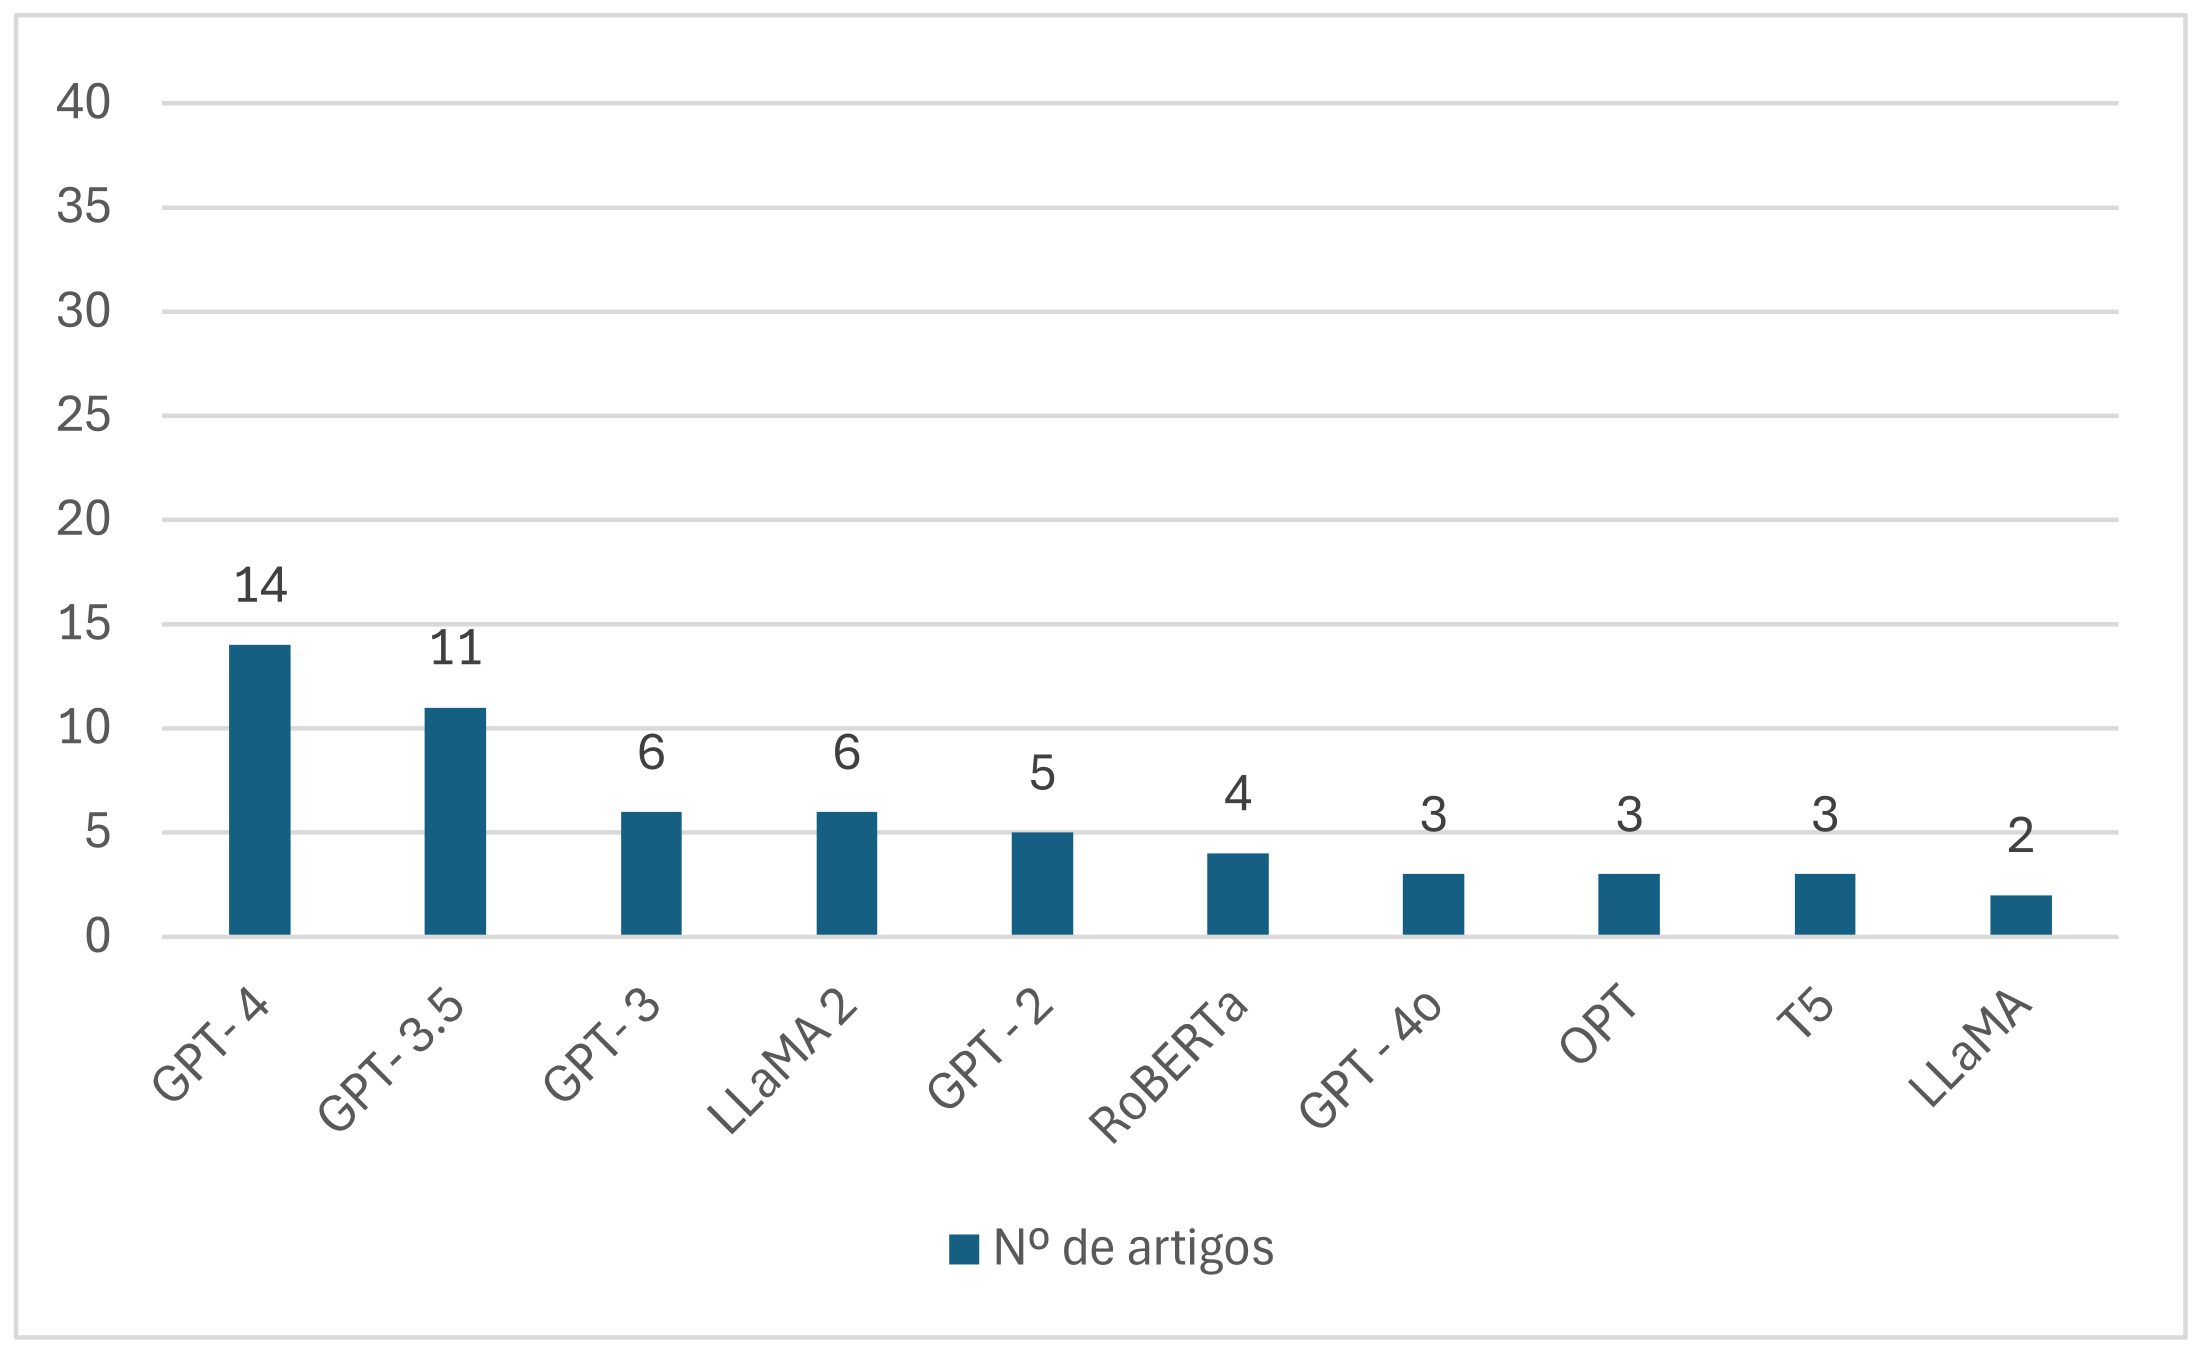
\includegraphics[width=\textwidth]{Imagens/fig-005.png}
\caption{Top 10 LLMs mais utilizados nos artigos analisados.}
\label{fig-5}
\source{Elaborado pelos autores.}
\end{minipage}
\end{figure}

A análise dos dados extraídos da revisão sistemática demonstra amplo uso de modelos da família GPT. O GPT-4 aparece como o modelo mais recorrente, utilizado em 14 dos 41 artigos analisados (34,1\%), seguido pelo GPT-3.5, presente em 11 publicações (26,8\%). A soma dessas duas versões representa mais da metade dos usos identificados, sinalizando uma preferência clara da comunidade científica por arquiteturas de última geração, capazes de oferecer maior acurácia e sofisticação na geração e análise de linguagem natural.

Outros modelos da mesma família também se destacam: GPT-3 (6 menções), GPT-2 (5) e, mais recentemente, o GPT-4o (3), indicando tanto a longevidade quanto a atualização contínua da família GPT no ecossistema acadêmico. A escolha frequente por esses modelos pode ser atribuída à sua ampla documentação, acessibilidade via APIs comerciais (como OpenAI), e à sua robustez para tarefas abertas e não estruturadas -- características especialmente relevantes para estudos que envolvem narrativas, metáforas e estruturas discursivas complexas.

Modelos alternativos também aparecem entre os mais utilizados, como LLaMA 2 (6 menções), RoBERTa (4), OPT (3), T5 (3) e LLaMA (2). Essa presença diversificada sugere o surgimento de um segundo grupo de modelos com características técnicas distintas, muitas vezes voltados a tarefas mais específicas ou com maior abertura para customização -- aspecto fundamental para pesquisadores que atuam com perspectivas metodológicas exploratórias ou críticas, como a análise hermenêutica ou estruturalismo narrativo.

Entre os 41 artigos analisados, destacam-se alguns trabalhos pela relevância e impacto nos avanços do uso de LLMs em criatividade, interpretação figurativa e explicabilidade:

\begin{itemize}
    \item ``On the creativity of large language models'' \cite{franceschelli2024} se sobressai ao discutir, sob a ótica das teorias de Margaret Boden, os desafios e oportunidades da criatividade em LLMs, abordando tanto aspectos filosóficos quanto éticos e sociais do uso dessas ferramentas em escrita criativa e seu impacto nas indústrias culturais.
    \item ``A Confederacy of Models: a Comprehensive Evaluation of LLMs on Creative Writing'' \cite{gomez-rodriguez2023} é outro destaque, ao realizar uma avaliação comparativa robusta entre múltiplos LLMs e escritores humanos, analisando, critérios como imaginação, coerência, estilo e originalidade, e evidenciando as limitações dos modelos em humor e criatividade genuína.
    \item No campo da compreensão figurativa, ``Large Language Model Displays Emergent Ability to Interpret Novel Literary Metaphors'' \cite{ichien2023} evidencia a capacidade emergente do GPT-4 em interpretar metáforas literárias, superando modelos anteriores. Por sua vez, ``Symbolic and Language Agnostic Large Language Models'' \cite{saba2023a} e ``Stochastic LLMs do not Understand Language'' \cite{saba2023b} são relevantes por questionarem as limitações subsimbólicas dos LLMs e proporem caminhos para modelos mais explicáveis e ontologicamente fundamentados.
    \item Finalmente, ``Metaphorian: Leveraging Large Language Models to Support Extended Metaphor Creation for Science Writing'' \cite{kim2023} e ``LLM-based multi-agent poetry generation in non-cooperative environments'' \cite{zhang2024} ilustram aplicações inovadoras dos LLMs na geração criativa, seja para metáforas científicas ou poesia, demonstrando avanços metodológicos e resultados superiores em diversidade e originalidade.
\end{itemize}

A Figura \ref{fig-6} sintetiza a distribuição temática identificada nos 41 artigos analisados, refletindo a frequência com que determinadas categorias emergem na literatura científica recente. Cada eixo do gráfico representa uma dimensão temática associada ao uso de linguagem figurada, criatividade, analogias, metáforas e raciocínio pragmático em contextos envolvendo LLMs.

A análise evidencia uma concentração significativa de estudos em torno da escrita criativa (11 artigos), seguida por investigações voltadas à detecção, geração e compreensão de metáforas (10 artigos), bem como à compreensão de linguagem figurada de maneira mais ampla (8 artigos). Esses achados sugerem que o campo tem direcionado seus esforços para temas vinculados à criatividade textual e ao tratamento computacional de metáforas.

Em contraste, tópicos como inferência simbólica, geração e resolução de analogias, além da problematização de limitações semânticas, coerência e outros aspectos relacionados, aparecem com baixa representatividade (entre 1 e 2 artigos). Tal distribuição indica uma lacuna nas investigações sobre processos inferenciais e estruturas simbólicas mais complexas, o que pode apontar para oportunidades futuras de pesquisa nesse domínio.

%--- código da figura 6 ---%
\begin{figure}[htbp]
\centering
\begin{minipage}{0.95\textwidth}
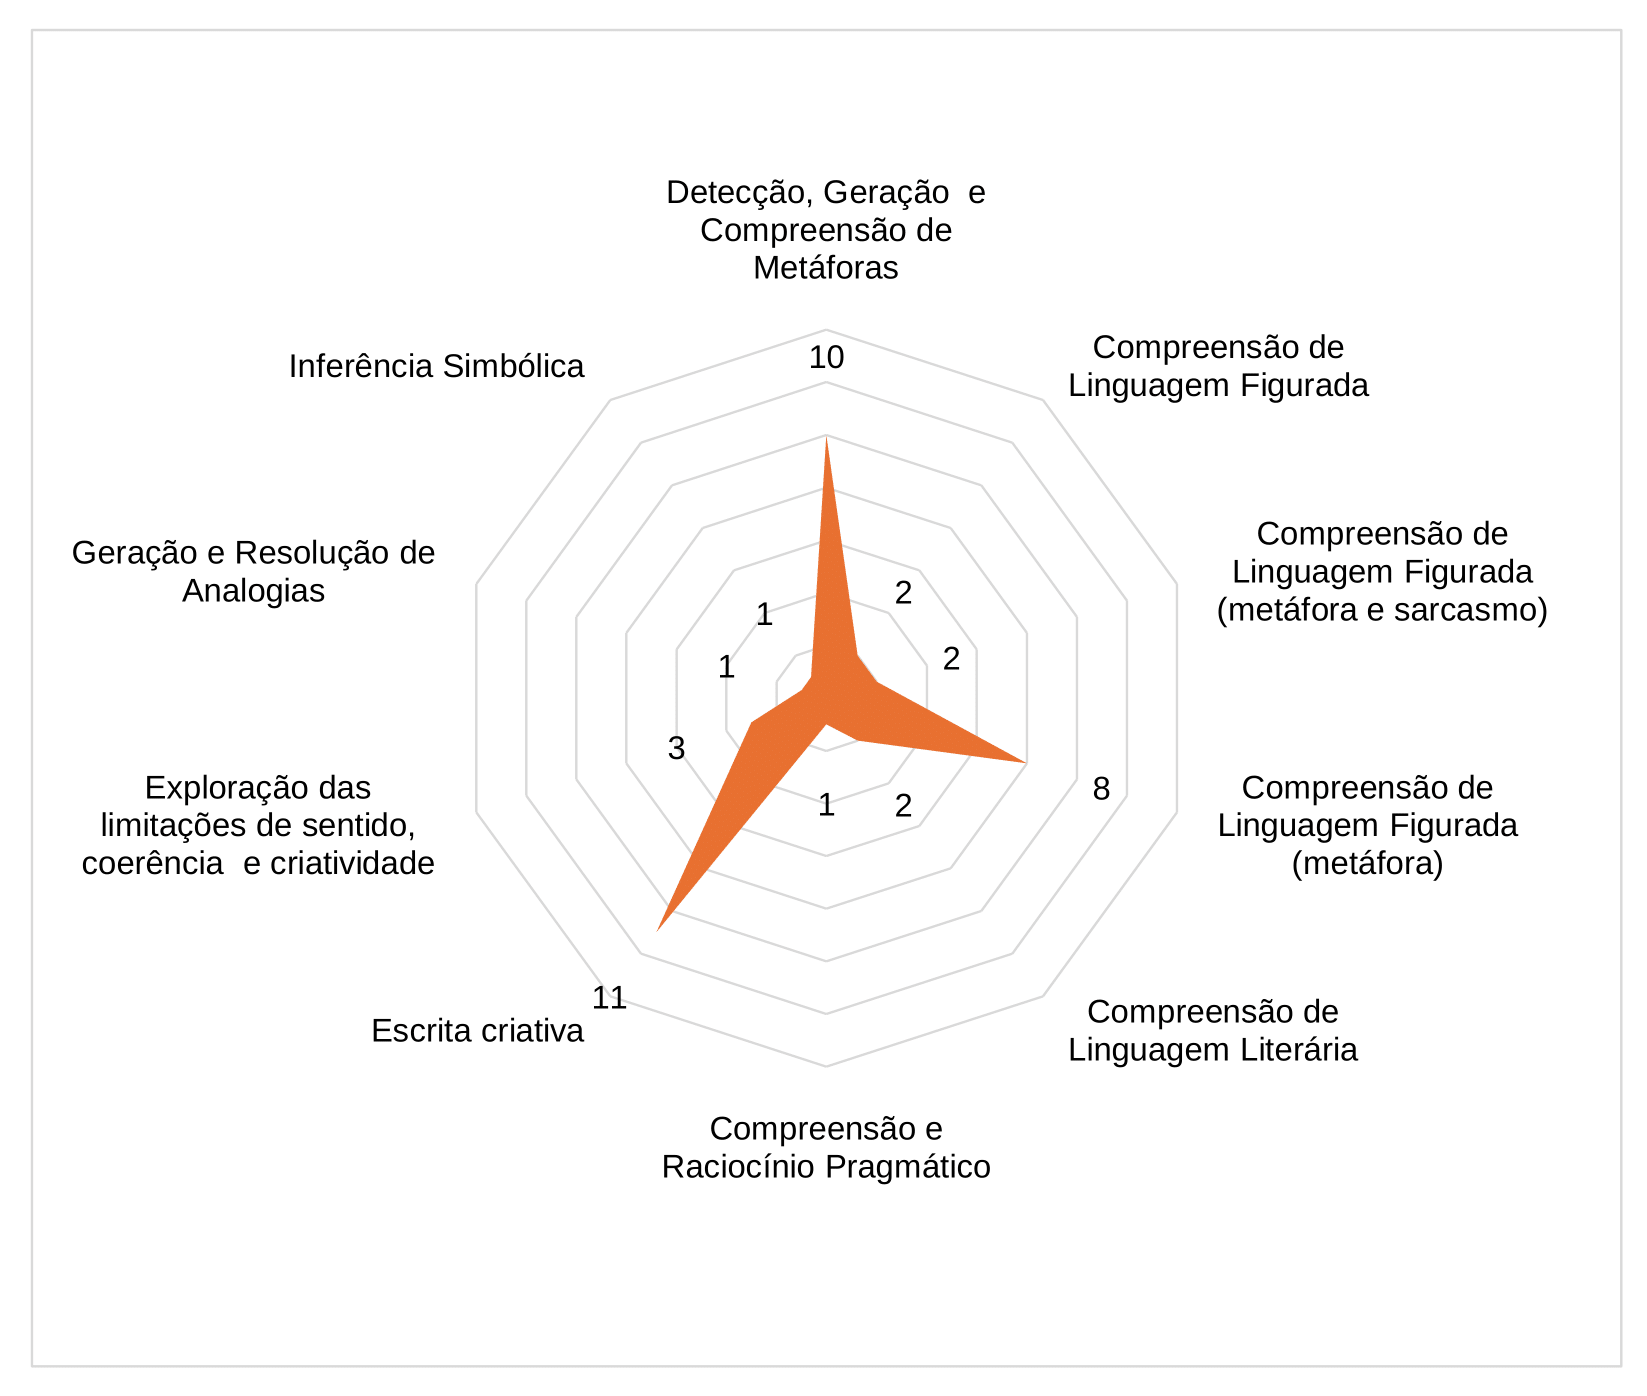
\includegraphics[width=\textwidth]{Imagens/fig-006.png}
\caption{Distribuição temática dos estudos sobre linguagem figurada, criatividade e raciocínio pragmático em LLMs (2014–2024).}
\label{fig-6}
\source{Elaborado pelos autores.}
\end{minipage}
\end{figure}

A Tabela \ref{tab-3} apresenta os principais objetivos identificados nos 41 artigos analisados. Algumas publicações abordam múltiplos objetivos, mas são categorizadas conforme o foco principal declarado por seus autores.

Os objetivos foram agrupados em grandes correlações temáticas, com indicação do número de artigos, percentual em relação ao total e destaques qualitativos. Essas características refletem tendências e lacunas observadas, como a busca por uma maior explicabilidade e criatividade nos LLMs.

%--- código da tabela 3 ---%
\begin{table}[h!]
\centering
\begin{threeparttable}
\caption{Análise cruzada dos objetivos dos 41 artigos sobre LLMs: correlações, frequências e destaques (2014--2024).}
\label{tab-3}
\small
\begin{tabular}{p{4cm} p{2cm} p{2cm} p{5cm}}
\toprule
Correlação temática & Nº de artigos & Percentual & Destaques \\
\midrule
Compreensão e Detecção de Metáforas & 18 & 44\% & Ênfase em \textit{frameworks} para identificação, \textit{datasets} para \textit{benchmark}, uso de LLMs para detecção e explicação de metáforas, desafios de transparência e autojulgamento. \\

Geração Criativa (Poesia, Narrativa, Roteiro) & 11 & 27\% & LLMs aplicados na geração de poesia, contos, roteiros e títulos; avaliação comparativa com humanos; destaque para criatividade, diversidade e originalidade. \\

Explicabilidade, Simbolismo e Aprendizagem Simbólica & 5 & 12\% & Discussão sobre limitações subsimbólicas dos LLMs, propostas de integração de abordagens simbólicas para maior explicabilidade e raciocínio transparente. \\

Análise de Estilo, Emoção e Idiomatismo & 4 & 10\% & Avaliação da interpretação de metáforas, sarcasmo, linguagem figurativa e emoções em contextos específicos como engenharia de \textit{software} e educação. \\

Aplicações em Educação e Alfabetização Crítica em IA & 3 & 7\% & Uso de LLMs para promover alfabetização digital, análise literária e compreensão crítica dos impactos sociais e éticos da IA. \\
\addlinespace
Total & 41 & 100\% & \\ 
\bottomrule
\end{tabular}
\source{Elaborado pelos autores.}
\end{threeparttable}
\end{table}

A análise das correlações temáticas nos 41 artigos selecionados permite identificar não apenas os objetivos recorrentes, mas também os principais desafios metodológicos, contribuições epistemológicas e possibilidades futuras no campo de estudo que articula LLMs com referenciais simbólicos, narrativos e do imaginário literário.

As abordagens identificadas demonstram um predomínio de investigações experimentais e comparativas, centradas na interpretação e geração de linguagem figurada. As técnicas mais comuns envolvem \textit{fine-tuning} de modelos pré-treinados, uso de \textit{prompt engineering} e integração de ferramentas semânticas externas (como ontologias e \textit{embeddings} especializados).

Os estudos indicam que, apesar dos avanços significativos dos modelos, sua capacidade simbólica ainda é dependente da curadoria humana, seja na criação de \textit{prompts} ou na avaliação dos resultados. As categorias de detecção de metáforas e geração criativa destacam um interesse em investigar os limites criativos dos LLMs, posicionando-os como agentes discursivos aptos a atuar em ambientes tradicionalmente humanos.

Entre os principais desafios destacam-se:  interpretabilidade e explicabilidade limitada em raciocínio simbólico complexo; transparência insuficiente em processos decisórios, especialmente em contextos ambíguos; fragilidade cultural na detecção de nuances contextuais; \textit{datasets} inadequados para diversidade semântica humana; e ausência de protocolos unificados para avaliação da criatividade computacional. Apesar das limitações, há diversas oportunidades promissoras: modelos híbridos simbólicos-conexionistas; aplicações educacionais para alfabetização crítica em IA; geração literária especializada por gêneros específicos; e métricas interdisciplinares baseadas em linguística, semiótica e estética.

Por fim, observam-se algumas lacunas relevantes: predominância de estudos em inglês e em contextos europeus  e norte-americanos, a ausência de análises da evolução dos LLMs, e a desconexão teórica entre produção técnica e as ciências humanas.

\section{Conclusão}
Esta revisão sistemática permitiu mapear e analisar criticamente as abordagens, desafios e oportunidades identificadas na literatura acadêmica (2014- 2024) sobre o uso de Grandes Modelos de Linguagem (LLMs) associados a referenciais simbólicos, narrativos e do imaginário literário. Os 41 artigos selecionados revelam um campo em consolidação, marcado por tensões entre os avanços técnicos e as limitações interpretativas dos modelos de linguagem quando aplicados em domínios complexos de significação.

Do ponto de vista das abordagens, constatou-se predominância de estudos voltados à geração criativa de textos e à detecção de linguagem figurada, em especial metáforas. A presença crescente de experimentos com técnicas híbridas — que combinam estruturas simbólicas e subsimbólicas — reforça o reconhecimento das limitações semânticas dos modelos puramente conexionistas. Ainda assim, observa-se que os LLMs têm possibilitado experimentações relevantes no campo da criatividade computacional, com contribuições não apenas técnicas, mas também epistemológicas.

Os principais desafios enfrentados referem-se à baixa interpretabilidade dos modelos, à dificuldade na captura de contextos culturais e ao \textit{déficit} de transparência nos processos de raciocínio linguístico. Em muitos casos, os estudos evidenciam que a mediação humana permanece indispensável, seja na curadoria de entradas, seja na validação dos \textit{outputs} gerados. Há também carência de metodologias avaliativas que articulem critérios quantitativos e qualitativos de forma robusta, especialmente no que se refere à criatividade textual.

A geração literária automatizada, quando pensada como ferramenta complementar e não substitutiva, pode apoiar práticas criativas, editoriais e didáticas. Além disso, a articulação entre modelos simbólicos e conexionistas desponta como agenda promissora para o futuro dos estudos de linguagem e cognição computacional.

Entre as lacunas observadas, destaca-se a baixa representatividade de idiomas e contextos culturais não hegemônicos, limitando a aplicabilidade global dos achados. Da mesma forma, nota-se uma distância teórica entre os aportes das ciências humanas -- especialmente da filosofia da linguagem, da semiótica e da teoria literária -- e os estudos mais técnicos sobre LLMs, comprometendo a densidade crítica de parte da produção analisada.

Como encaminhamento, recomenda-se que pesquisas futuras:

\begin{itemize}
    \item Diversifiquem contextos geográficos e linguísticos;
    \item Desenvolvam protocolos avaliativos unificados;
    \item Integrem abordagens técnicas e humanísticas;
    \item Implementem métricas interdisciplinares robustas;
    \item Promovam modelos híbridos explicáveis.
\end{itemize}

Assim, os resultados desta revisão contribuem para compreender os rumos da pesquisa sobre LLMs aplicados ao imaginário literário e referenciais simbólicos, apontando tanto seus limites atuais quanto os caminhos possíveis para uma inteligência artificial mais interpretável, ética e culturalmente contextualizada.

\section*{Financiamento}
Coordenação de Aperfeiçoamento de Pessoal de Nível Superior (CAPES).



\printbibliography\label{sec-bib}
% if the text is not in Portuguese, it might be necessary to use the code below instead to print the correct ABNT abbreviations [s.n.], [s.l.]
%\begin{portuguese}
%\printbibliography[title={Bibliography}]
%\end{portuguese}


%full list: conceptualization,datacuration,formalanalysis,funding,investigation,methodology,projadm,resources,software,supervision,validation,visualization,writing,review
\begin{contributors}[sec-contributors]
\authorcontribution{Patrick Fernandes Rezende Ribeiro}[conceptualization,datacuration,formalanalysis,investigation,writing,review]
\authorcontribution{Denise Fukumi Tsunoda}[conceptualization,methodology,projadm,supervision,validation,review]
\end{contributors}


\end{document}

